\cptr{Parameter estimation and Bayes factors}
{Parameter estimation and Bayes factors}
{Jeffrey N.\ Rouder, Julia Haaf, and Joachim Vandekerckhove}

Bayesian analysis has become increasing popular in many fields including psychological science.  There are many advantages to the Bayesian approach.  Some champion its clear philosophical underpinnings where probability is treated as a statement of belief or information and the focus is on updating beliefs rationally in face of new data \cite{deFinetti:1974,Edwards:etal:1963}.  Others note the practical advantages---Bayesian analysis often provides a tractable means of solving difficult problems that remain intractable in more conventional frameworks \cite{Gelman:etal:2004}.  This practical advantage is especially pronounced in psychological science where substantive models are designed to account for mental representation and processing.  As a consequence, the models tend to be complex and nonlinear, and may include multiple sources of variation \cite{Kruschke:2011a,Lee:Wagenmakers:2013,Rouder:Lu:2005}.  Bayesian analysis, especially Bayesian nonlinear hierarchical modeling, has been particularly successful at providing straightforward analyses in these otherwise difficult settings \cite<e.g.,>{Rouder:etal:2003,Vandekerckhove:etal:2011}.  

Bayesian analysis is not a unified field, and Bayesian analysts disagree with one another in important ways.\footnote{Perhaps such disagreements should be expected given the contentious history of academic statistics.  Even null hypothesis significance testing is a contentious hybrid of Fisherian and Neyman-Pearson schools of thought \cite{Gigerenzer:etal:1989,Lehmann:1993}.}   We highlight here two popular Bayesian approaches that seem incompatible and discuss them in the context of the simple problem of determining whether performance in two experimental conditions differs.  In one approach, termed here the \textbf{posterior-estimation approach}, the difference between the conditions is represented by a parameter, and posterior distributions about this parameter are updated using Bayes' Rule.  From these posterior distributions, researchers may observe directly which parameter values are plausible, and, as importantly, which are implausible.  Two examples are provided in Figure~\ref{k:fig}.  In Figure~\ref{k:fig}A the posterior distribution is compact in extent and localized away from zero, and this localization serves as evidence for a statistically substantial difference between the two conditions.  In Figure~\ref{k:fig}B, in contrast, the value of zero is well within the belly of posterior, indicating that there is little evidence for such a difference.  Perhaps the leading advocate of the posterior-estimation approach in psychology is Kruschke \cite{Kruschke:2011,Kruschke:2012}.  Although the posterior-estimation approach seems straightforward, it is not recommended by a number of Bayesian psychologists including \citeA{Dienes:2014}, \citeA{Gallistel:2009}, \citeA{Rouder:etal:2009a}, and \citeA{Wagenmakers:2007}.  These authors instead advocate a \textbf{Bayes factor} approach.  In Bayesian analysis, it is possible to place probability on models themselves without recourse to parameter estimation.   In this case, a researcher could construct two models: one that embeds no difference between the conditions and one that embeds some possible difference.  The researcher starts with prior beliefs about the models and then updates these rationally with Bayes' rule to yield posterior beliefs.  Evidence from data is how beliefs about the models themselves change in light of data; there may be a favorable revision for either the effects or null-effects model.

\begin{figure}
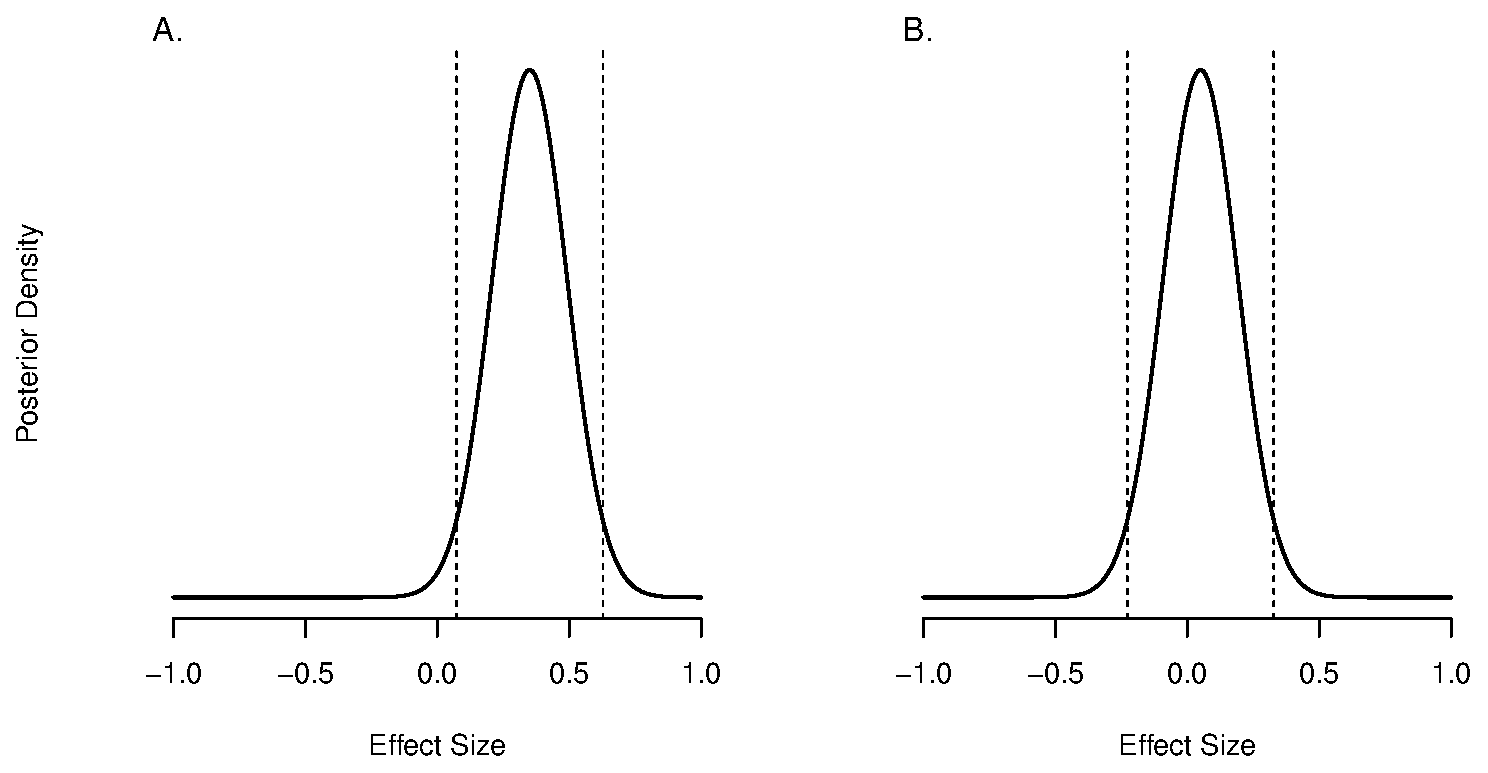
\includegraphics[width=\textwidth]{figs/bi4_fig1}
\caption{In the posterior-estimation approach, the posterior distribution describes which parameter values are plausible and implausible.  \textbf{A.} The posterior localizes the effect away from zero perhaps providing evidence for an effect.  \textbf{B.} The posterior localizes the effect around zero perhaps providing a lack of evidence for an effect.  Dashed lines indicate the 95\% credible intervals on posteriors.}
\label{k:fig}
\end{figure}

Posterior estimation and Bayes factor approaches do not necessarily lead to the same conclusions.  Consider for example the posterior in  Figure~\ref{k:fig}A where the posterior credible interval does not include zero.  This posterior seemingly provides positive evidence for an effect.  Yet, the Bayes factor, which is discussed at length subsequently, is 2.8-to-1 in favor of the effect.  If we had started with 50-50 beliefs about an effect (vs. a lack of an effect), we end up with just less than 75-25 beliefs in light of data.  While this is some revision of belief, this small degree is considered rather modest \cite{Jeffreys:1961,Raftery:1995} rather than substantial.

This divergence leaves the nonspecialist in a quandary about whether to use posterior estimation or Bayes factors.  We fear this may lead some to ignore Bayesian analysis altogether.  Here we address this quandary head-on:  We will first draw a sharp contrast between the two approaches and show that they provide for quite different views of evidence.  Then, to help understand these differences, we provide a unification.  We show that the Bayes factor may be represented as estimation under a certain model specification known in the statistics literature as a {\em spike-and-slab} model \cite{George:McCulloch:1993}.  With this demonstration, one difference between estimation and a Bayes factor approach comes into full view---it is a difference in model specification rather than any deep difference in the Bayesian machinery.  These spike-and-slab models entail different commitments than more conventional models.  Our own view is that the commitments underlying spike-and-slab are the correct ones for most testing questions.    Once researchers understand these commitments, they can make informed and thoughtful choices about which are most appropriate for specific research applications.  

\section{Posterior Estimation}

Bayesian estimation is performed straightforwardly through updating by Bayes' rule.  Let us take a simple example where a set of participants provide performance scores in each of two conditions.  For example, consider a priming task where the critical variable is the response time, and participants provide a mean response time in a primed and unprimed condition.  Each participant's data may be expressed as a difference score, namely the difference between mean response times.  Let $Y_i$, $i=1,\ldots,n$ be these difference scores for $n$ participants.  In the usual analysis, researchers would perform a $t$-test to assess whether these difference scores are significantly different from zero.

Bayesian analysis begins with consideration of a model, and in this case, we assume that each difference score is a draw from a normal with mean $\mu$ and variance $\sigma^2$:
\begin{equation}
Y_i \sim \mbox{Normal}(\mu,\sigma^2), \;\;\; i=1,\ldots,n.
\end{equation}
In the following development, we will assume that $\sigma^2$ is known to simplify the exposition, but it is straightforward to dispense with this assumption.  It is helpful to consider the model in terms of effect sizes, $\delta$, where $\delta=\mu/\sigma$ is the true effect size and is the parameter of interest.  

Bayesian analysis proceeds by specifying beliefs about the effect-size parameter $\delta$.  The beliefs are expressed as a prior distribution on parameters.  In this article, we use the term {\em prior} and {\em model} interchangeably as a prior is nothing more than a model of parameters.  Model $\calM_1$ provides prior beliefs on $\delta$.
\begin{eqnarray} \label{M1}
\calM_1: &&\delta \sim \mbox{Normal}(0,\sigma_0^2).
\end{eqnarray}
The centering of the distribution at zero is interpreted as a statement of prior equivalence about the direction of any possible effect---negative and positive effects are {\em a priori} equally likely.  The prior variance, $\sigma_0^2$ must be set before analysis, and it is helpful to explore how the value of this setting affects estimation.  Figure~\ref{sig0}A shows this effect.  Ten hypothetical values of $Y_i$, the difference scores, are shown as line segments across the bottom of the plot.  The sample mean of these ten is shown as the vertical line.   The posterior distributions of $\delta$ are shown for three different prior settings.  The first prior setting, $\sigma_0=.5$, codes an {\em a priori} belief that $\delta$ is not much different than zero.  The second prior setting, $\sigma_0=2$, is a fairly wide setting that allows for a large range of reasonable effect sizes without mass on exceedingly large values.  The third prior setting, $\sigma_0=5000$ indicates that researcher is unsure of the effect size, and holds the possibility that it can be exceedingly large.   Even though the priors are quite different, the posterior distribution are quite similar.   We may say that the posterior is robust to wide variation in prior settings.  In fact, it is possible to set $\sigma_0=\infty$ to equally weight all effect sizes {\em a priori},  and in this case, the posterior would be indistinguishable from that for $\sigma_0=5000$.  This robustness to prior settings may be viewed by some as an advantage of Model $\calM_1$ on  $\delta$.  As will be shown, while this robustness holds for $\calM_1$, it is not a general property of Bayesian estimation.  We will introduce a useful model in the next section where it does not hold.

\begin{figure}
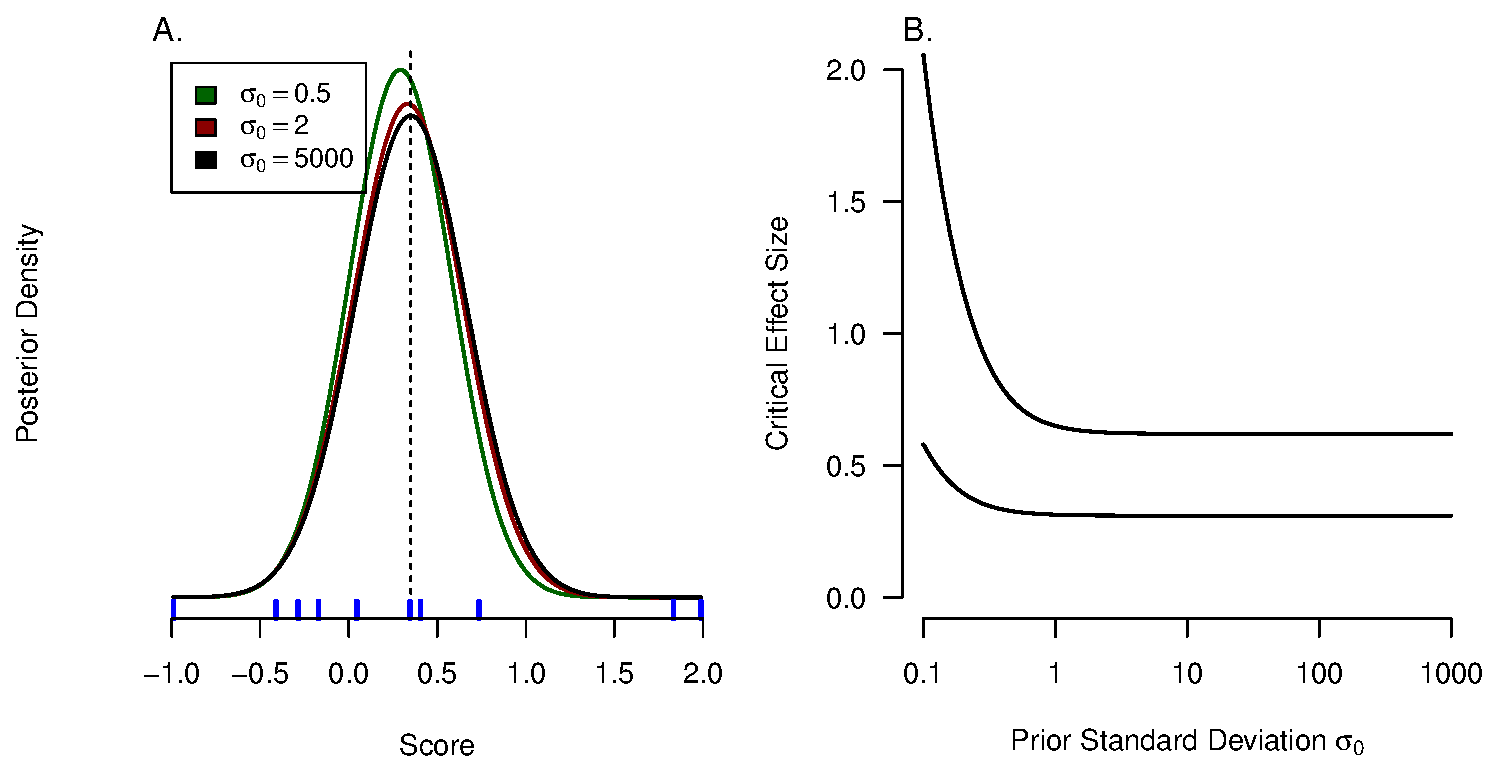
\includegraphics[width=\textwidth]{figs/bi4_fig2}
\caption{The dependence of the posterior estimation on prior setting $\sigma_0$.  \textbf{A.} Posterior distributions on effect size $\delta$ for $N=10$ and for a sample effect size of .35. for three settings of $\sigma_0$ \textbf{B.} Minimum observed effect sizes needed such that the posterior 95\% credible interval excludes zero.  The two lines are for sample sizes of 10 (top) and 40 (bottom).  The results show a robustness to the prior setting of $\sigma_0$. }
\label{sig0}
\end{figure}

There are many ways to use the posterior distributions to state conclusions.  One could simply inspect them and interpret them as needed (Gelman \& Shalizi, 2013 and Rouder et al., 2008 take variants of this approach). \nocite{Rouder:etal:2008d,Gelman:Shalizi:2013} Alternatively, one could make a set of inferential rules.  In his early career, \citeA{Lindley:1965} recommended inference by {\em highest-density credible intervals} (HDCIs).  These highest-density credible intervals  contain a fixed proportion of the mass, say 95\%, and posterior values inside the interval are greater than those outside the interval.  
Example of these HDCIs are shown in Figure~\ref{k:fig} with the dashed vertical lines.  Values outside the intervals may be considered sufficiently implausible to be untenable.  By this reasoning, there is evidence for an effect in Figure~\ref{k:fig}A as zero is outside the 95\% credible interval.  Figure~\ref{sig0}B shows that inference by credible intervals does not depend heavily on the prior setting $\sigma_0^2$.  Shown is the minimal effect size needed such that zero is excluded from the lower end of the credible interval.  As can be seen, this value stabilizes quickly and varies little.   

\citeA{Kruschke:2012} takes a similar approach.  A posterior interval may be compared to a pre-established region, called a {\em region of practical equivalence} or ROPE.   ROPES are small intervals around zero that are considered to be practically the same as zero.  An example of a ROPE might be the interval on effect sizes from $-.2$ to $.2$. In Kruschke's approach, one concludes that the null hypothesis is false if the HDCI falls completely outside of the ROPE. If the HDCI falls completely inside of the ROPE, one concludes that the null hypothesis is (for all practical purposes) true.  If the HDCI partly overlaps with the ROPE, Kruschke recommends one reserve judgment.  Inferences drawn this way are robust to the prior setting of $\sigma_0$, and arbitrarily large (even infinite) values may be chosen.

\section{Bayes Factors}
The contrasting approach is inference by Bayes factors.  In Bayesian analysis, it is possible to place beliefs directly onto models themselves and update these beliefs with Bayes' rule.  Let $\calM_A$ and $\calM_B$ denote any two models.  Let $Pr(\calM_A)$ and $Pr(\calM_B)$ be {\em a priori} beliefs about the plausibility of these two models.  It is more desirable to state relative beliefs about the two models as odds.  The ratio $Pr(\calM_A)/Pr(\calM_B)$ is the relative plausibility of the models, and for example, the statement $Pr(\calM_A)/Pr(\calM_B)=3$ indicates that Model $\calM_A$ is three times as plausible as Model $\calM_B$.  Odds such as $Pr(\calM_A)/Pr(\calM_B)$ are called {\em prior odds} because they are stipulated before seeing data.  They may be contrasted to {\em posterior odds}, which are the same odds in light of the data and denoted  $Pr(\calM_A \mid \bfY)/Pr(\calM_B \mid \bfY)$. be the prior and posterior odds, respectively. Bayes rule for updating to posterior odds from prior odds is
\begin{equation}\label{eq:bf}
\frac{Pr(\calM_A)}{Pr(\calM_B)} = \frac{f(\bfY \mid \calM_A)}{f(\bfY \mid\calM_B)} \times \frac{Pr(\calM_A)}{Pr(\calM_B)}.
\end{equation}
The updating factor, $f(\bfY | \calM_A)/f(\bfY | \calM_B)$, is called the {\em Bayes factor}, and it  describes how the data have led to a revision of beliefs about the models.  Several authors including \cite{Jeffreys:1961} and \citeA{Morey:etal:2016} refer to the Bayes factors as the {\em strength of evidence from data about the models} precisely because the strength of evidence should refer to how data lead to revision of beliefs.  The Bayes factor has a second meaning stemming from it being the relative probability of data under models.  The probability of data under a model may be thought of as the predictive accuracy of that model -- the degree to which the model predicted the data.  The data in the equation is the observed date we obtain in an experiment, and if if the probability of observed data is high, then the model predicted the observed data to be where they were observed.  If the probability of data is low, then the model did not predicted the observations well.  The Bayes factor is the relative predictive accuracy of one model relative to another.  The deep meaning of Bayes' rule is that the strength of evidence is the \emph{relative predictive accuracy}, and this is captured by the Bayes factor in Equation~\ref{eq:bf}.

We denote the Bayes factor by $B_{AB}$, where the subscripts indicate which two models are being compared. 
A Bayes factor of $B_{AB}=10$ means that prior odds should be updated by a factor of 10 in favor of model $\calM_A$; likewise, a Bayes factor of $B_{AB}=.1$ means that prior odds should be updated by a factor of 10 in favor of model $\calM_B$. Bayes factors of $B_{AB}=\infty$ and $B_{AB}=0$ correspond to infinite---total---support of one model over the other with the former indicating infinite support for model $\calM_A$ and the latter indicating infinite support for model $\calM_B$.  

For the simple example of comparing performance in two experimental conditions, we need one model for an effect a different model for a lack of an effect (which is also called an invariance).  A suitable model for an effect is the previous model, $\calM_1$ given in (\ref{M1}).  A model for an invariance is given by 
\begin{eqnarray*}
\calM_0: && \delta = 0.
\end{eqnarray*}
With this setup, the Bayes factor is straightforward to compute.\footnote{The Bayes factor between Model $\calM_1$ and $\calM_0$ is 
\begin{equation} \label{workingBF}
B_{10} = \frac{1}{\sqrt{n\sigma_0^2+1}}\exp\left(\frac{n^2 d^2}{2(n+1/\sigma_0^2)}\right)
\end{equation}
where $d$ is the observed effect size given by $\bar{Y}/\sigma$.}

\begin{figure}[!t]
\centering
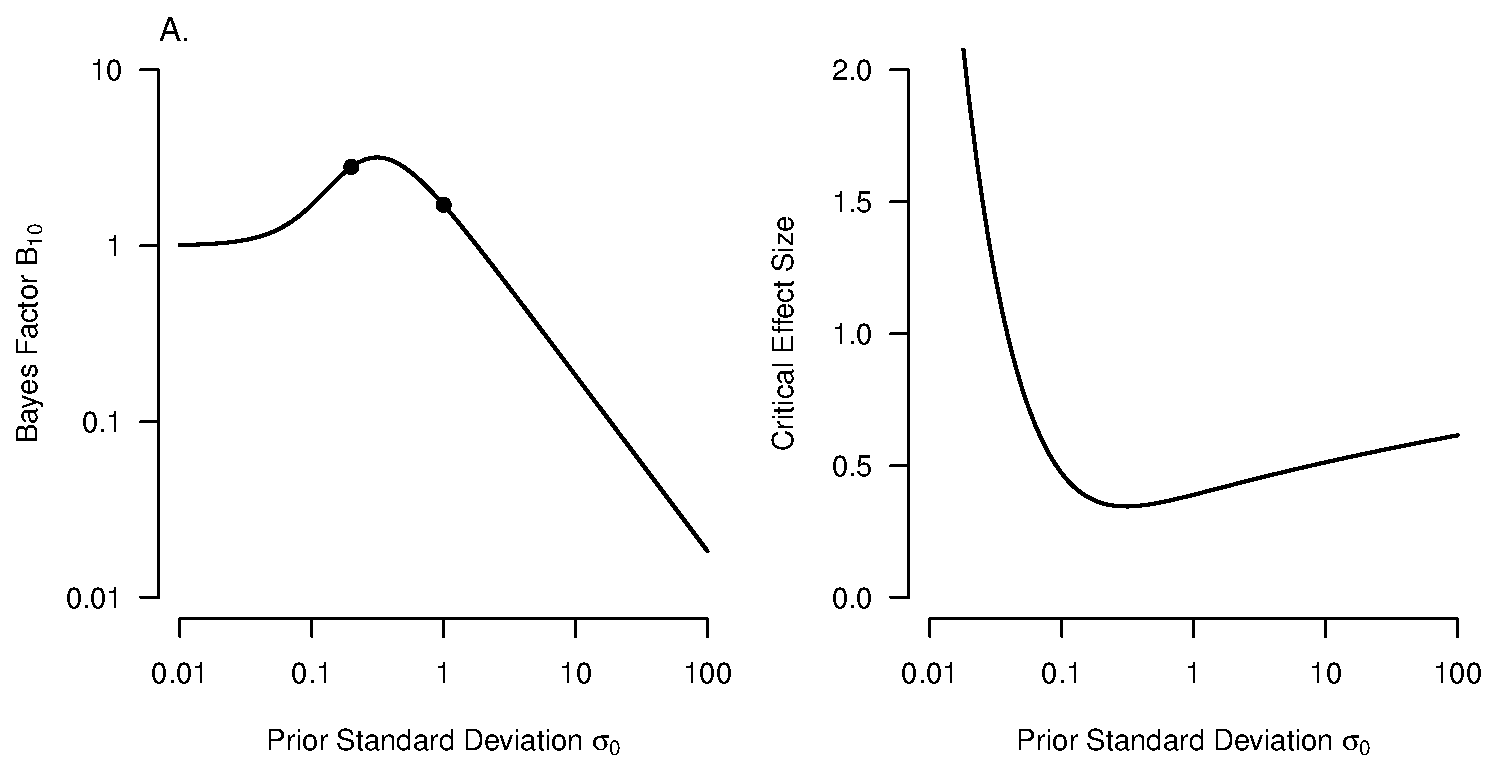
\includegraphics[width=\textwidth]{figs/bi4_fig3}
\caption{The dependence of Bayes factor on prior setting $\sigma_0$.  \textbf{A.} Bayes factor as a function of $\sigma_0$ for $N=40$ and for an observed effect size of .35 and a sample size of 40 observations.  \textbf{B.} Minimum observed effect sizes needed such that Bayes factor favors the alternative by 3-to-1.  The filled circles show the lower and upper bounds of reasonable variation in prior standard deviation. }
\label{fig:bi4:bf}
\end{figure}

Inference by Bayes factor is more dependent on the prior setting $\sigma^2_0$ than is inference by the preceding posterior-estimation approach.  Figure~\ref{fig:bi4:bf}A shows the effects of increasing $\sigma_0$. As can be seen, the Bayes factor $B_{10}$ favors the alternative when $\sigma_0$ is small (say, near 1) but decreases toward zero as $\sigma_0$ becomes increasingly large. Of note is the limit as $\sigma_0$ gets increasingly large.  These diffuse priors on effect size in the alternative leads to total support for the null model over the alternative \cite{Lindley:1957}, and this result contrasts to that for inference with credible intervals where inference reflects the data even when $\sigma_0$ becomes increasingly large.  This result occurs because the Bayes factor is sensitive to the complexity of the model, and when the $\sigma_0^2=\infty$, the alternative can account for all data equally well, without constraint.  Consequently, it is penalized completely.  Figure~\ref{fig:bi4:bf}B provides an different view of the effect of prior setting $\sigma_0$.  It shows the minimum positive effect size need to support a Bayes factor of 3-to-1 in favor of Model $\calM_1$ over $\calM_0$ and is comparable to Figure~\ref{sig0}B.  As can be seen, inference by Bayes factor is more sensitive to prior settings than inference by estimation. 

At first glance, this dependence of the Bayes factors on the prior settings may seem undesirable.  One fear is that researchers can seemingly obtain different results by adjusting the prior settings perhaps undermining the integrity of their conclusions.  This dependence seems all the more undesirable when contrasted to the the robustness of posterior intervals to prior settings as shown in Figure~\ref{sig0}.  However, the situation is far more nuanced, and we believe researchers should not worry too much about prior dependence or lack thereof.  Indeed both Bayesian parameter estimation and Bayes factor model selection are supported by the same rules of probability (see Etz \& Vandekerckhove, this issue), and the differences are more subtle and perhaps even more interesting than they first appear.  In the next section we provide a unification, and with this unification can pinpoint the differences and make recommendations for researchers.

\section{Unification}

\begin{figure}[!t]
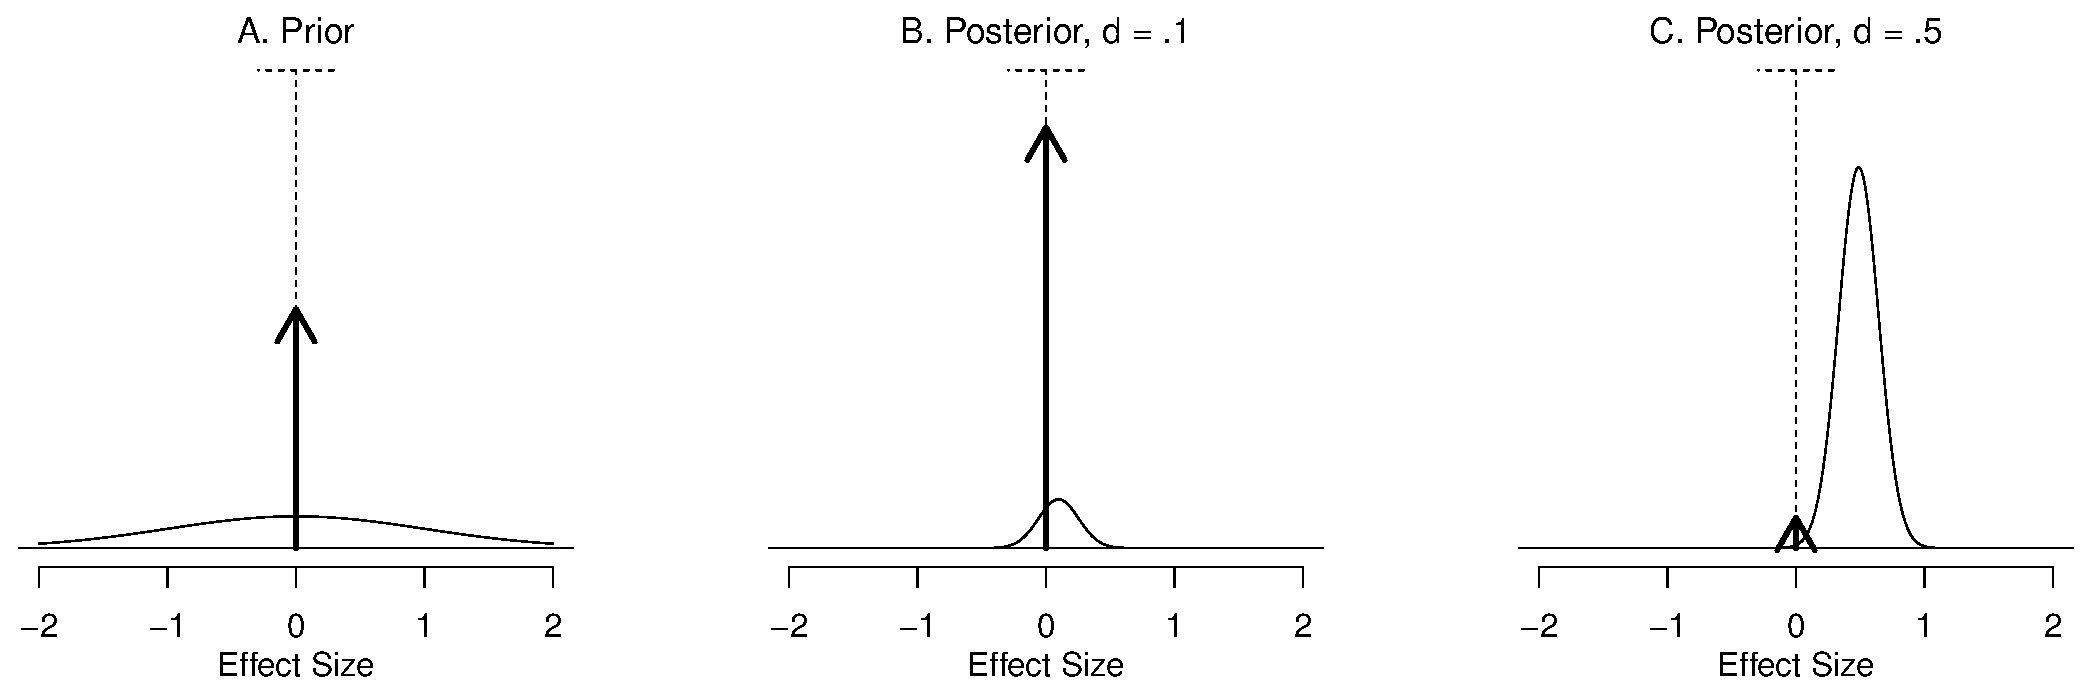
\includegraphics[width=\textwidth]{figs/bi4_fig4}
\caption{The spike-and-slab model is a mixture of a spike, shown as an arrow, and slab, shown as the normal curve.  \textbf{A.}  Prior distribution on effect size with half the mass in the spike, and the slab centered around zero.  \textbf{B-C.} The posterior on effect size $\delta$ for observed effect sizes of $d=.1$ and $d=.5$, respectively, for a sample size of 40.}
\label{fig:bi4:spikeSlab}
\end{figure}

The differences between the estimation and Bayes factor approach can be understood by combining models $\calM_0$ and $\calM_1$.  Figure~\ref{fig:bi4:spikeSlab}A shows the combination, which is expressed as a mixture.   One component of the mixture is the usual normal model on effect size (Model $\calM_1$), and this component is denoted by the curve in Figure~\ref{fig:bi4:spikeSlab}A.  The other component is a placing mass on the point of zero, and this component is denoted by the arrow.  In this case, the arrow is half-way up its scale, shown in dashed line, indicating that half of the total mass is placed at zero, and the other half is distributed around zero.  This model is well known in the statistics literature as a {\em spike-and-slab model} \cite{Mitchell:Beauchamp:1988}.  We denote it by Model $\calM_s$.\footnote{The density of a spike-and-slab model is given by 
\[
f(\delta) = \rho_0 s(\delta) + (1-\rho_0)\phi(\delta/\sigma_0),
\]
where $s$ is the density of the spike, defined next, $\phi$ is the density of a standard normal, $\rho_0$ is the prior mass on the spike, and $\sigma_0^2$ is the variance of the slab.   The density of the spike, $s$, is known as a Dirac delta function and defined as follows: Consider a normal density centered at zero with standard deviation $\eta$, denoted $g(\delta) = \phi (\delta/ \eta)$.   The Dirac delta function, $s$, is defined as the density in the limit that $\eta \rightarrow 0$:
\[
s(\delta) = \lim_{\eta \rightarrow 0} \phi \left( \frac{\delta}{\eta}\right) =
\left\{ \begin{array}{cc} \infty, & \delta=0,\\
0, & \mbox{otherwise.} \end{array} \right.
\]
}
The spike-and-slab model in Figure~\ref{fig:bi4:spikeSlab} has two parameters: the amount of probability in the spike, denoted $\rho_0$, and the variance of the slab, denoted $\sigma^2_0$.  Figure~\ref{fig:bi4:spikeSlab}A shows the case where $\rho_0=1/2$ and $\sigma_0^2=1$.  

It is straightforward  to update beliefs about $\delta$ in the spike-and-slab model using Bayes' rule.\footnote{The resulting posterior density, $f(\delta|\bfY)$  is 
\[
f(\delta | \bfY) = \rho_1 s(\delta) + (1-\rho_1)\phi\left(\frac{\delta-\mu_1}{\sigma_1}\right),
\]
where
\begin{eqnarray*}
\sigma^2_1 &=& (n+\sigma_0^{-2})^{-1}\\
\mu_1 &=& nd\sigma^2_1\\ 
\rho_1 &=& \frac{\rho_0}{\rho_0+(1-\rho_0)B_{01}},
\end{eqnarray*}
where $d$ is the observed effect size and $B_{01}$ is the Bayes factor between Model $\calM_0$ and $\calM_1$ .
}
Figure~\ref{fig:bi4:spikeSlab}B-C show a few examples for different observed effect sizes.  In all cases, the resulting posterior is in the spike-and-slab form, but the spike has changed mass and the slab has shifted and rescaled.  Figure~\ref{fig:bi4:spikeSlab}B shows the posterior for a small observed effect size of 0.1. The spike is enhanced as the effect is compatible with a null effect.  The slab is attenuated in mass, narrowed, and shifted form 0 to about .1.  Figure~\ref{fig:bi4:spikeSlab}B shows the posterior for a large observed effect size of 0.5.  The spike is attenuated as the effect is no longer compatible with the null, and the slab is enhanced, narrowed, and shifted from 0 to about .5.  
  
There is an intimate relationship between the spike-and-slab posterior distribution and the Bayes factor $B_{01}$ for the comparison between models $\calM_0$ and $\calM_1$: The Bayes factor describes the change in the spike.  The prior probability of the spike, $\rho_0$, can be expressed as odds, $\omega_0=\rho_0/(1-\rho_0)$.  The posterior probability of the spike, $\rho_1$, can likewise be expressed as odds, $\omega_1=\rho_1/(1-\rho_1)$.   The Bayes factor is the change in odds: $\omega_1/\omega_0$.   In Figure~\ref{fig:bi4:spikeSlab}B, for example, the initial odds on the spike were 1-to-1, indicating that equal mass was in the spike as was in the slab.  In light of data, the posterior odds were 7.4-to-1, or that 88\% of the posterior mass was in the spike and 12\% of posterior mass was in the slab.  Indeed, the Bayes factor for this case is $B_{01}=7.4$, and this factor describes the change in odds in the spike in light of data (because originally they were 1-to-1).

The spike-and-slab Model $\calM_s$ yields posterior estimates of effect size that behave differently, in fact more advantageously, than the slab-only estimates from $\calM_1$.  Figure~\ref{est}A-B shows the comparison.  The solid curves are posterior means of $\delta$ as a function of observed effect size $d$.  For the slab-only specification (Panel A), the estimated mean follows the observed value, and do so for all prior values of $\sigma^2_0$.   But, for the spike-and-slab specification ($\calM_s$, Panel B), there is a pull toward zero.  This pull is known as shrinkage.   Shrinkage is well known in hierarchical models and often results in estimates that have lower error and perform better out of sample\cite{James:Stein:1961,Efron:Morris:1977}.  The shrinkage from the spike-and-slab model is {\em adaptive} in that shrinkage toward zero is sizable for small observed values while there is hardly any shrinkage for large values.  The dynamics are that small observed effect sizes are more compatible with the hypothesis that there is no effect, and therefore, estimates are more influenced by the zero value.  Large effects in contrast are more compatible with the hypothesis that there as an effect, and the estimates are more influenced by the sample effect size.

Adaptive shrinkage is an exceedingly useful part of modern Bayesian analysis.  It is a Bayesian approach to variable selection, classification, and smoothing, and, as will be discussed, it has become popular in multivariate settings.  
The amount of adaptive shrinkage depends on the prior setting $\sigma^2_0$.  As $\sigma_0^2$ increases, there is more shrinkage to zero as the spike is relatively more salient.  In this regard, the prior setting $\sigma_0^2$ serves as a tuning parameter.

From the behavior of the effect-size estimate that we observe under the spike-and-slab specification, we can draw a few conclusions: First, estimation is made within the context of a specified model.  The model is important, and  the obtained \emph{parameter estimates are a function of the choice of model specification}.  Model estimates with the spike-and-slab prior show adaptive shrinkage -- effect size estimates are attenuated towards zero to an extent that depends on the probability of there being any effect at all.\footnote{The spike-and-slab model allows for an added level of flexibility in that we can inspect the parameter estimate \emph{in the slab by itself} provided that we are comfortable assuming---after seeing the posterior distribution that includes the spike and deciding that the spike mass can now safely be ignored---that there is an effect.  In Figure~\ref{fig:bi4:spikeSlab}C, we would arrive at the estimate $\hat{d} \approx 0.5$.}
Second, Bayesian parameter estimation is not in itself more robust to prior settings than the Bayes factor: \emph{Robustness to prior settings is a function of model specification.}

These consequences, that the value of estimates and their robustness to prior settings both depend critically on the model specification, hold for inferences drawn from credible intervals as well.  Figure~\ref{est}{C-E} show the comparison of credible intervals.  The shaded areas show the 95\% CIs as a function of observed effect size.  For the slab-only specification, the credible intervals maintain a constant width for all observed effect size values.  The key question is when does the credible interval include or exclude the value of zero.   The vertical dashed lines show transition points -- if the observed values are more extreme, then the 95\% CI does not include zero.  For the slab-only specification, the CIs include zero for observed effect sizes between -.325 and .325.  Values more extreme exclude zero, and by posterior estimation logic, these values lead ot a rejection of the null.   The spike-and-slab specifications results in different behavior for the credible intervals.  For extreme observed values, say those greater than .65 in magnitude, the CIs are quite similar to the slab-only specification.  For  less extreme values, the spike has influence, and the resulting 95\% CI often includes the value of zero.  As a result, the transition points are wider -- it takes more extreme observed values to localize the 95\% CI away from zero.  For when $\sigma_0=1$, the null may rejected only if the observed effect size is more extreme in magnitude than .55, which is quite a bit larger than the .325 for slab-only specification.  This value is increased to .585 when $\sigma_0=10$.  

\begin{figure}[!t]
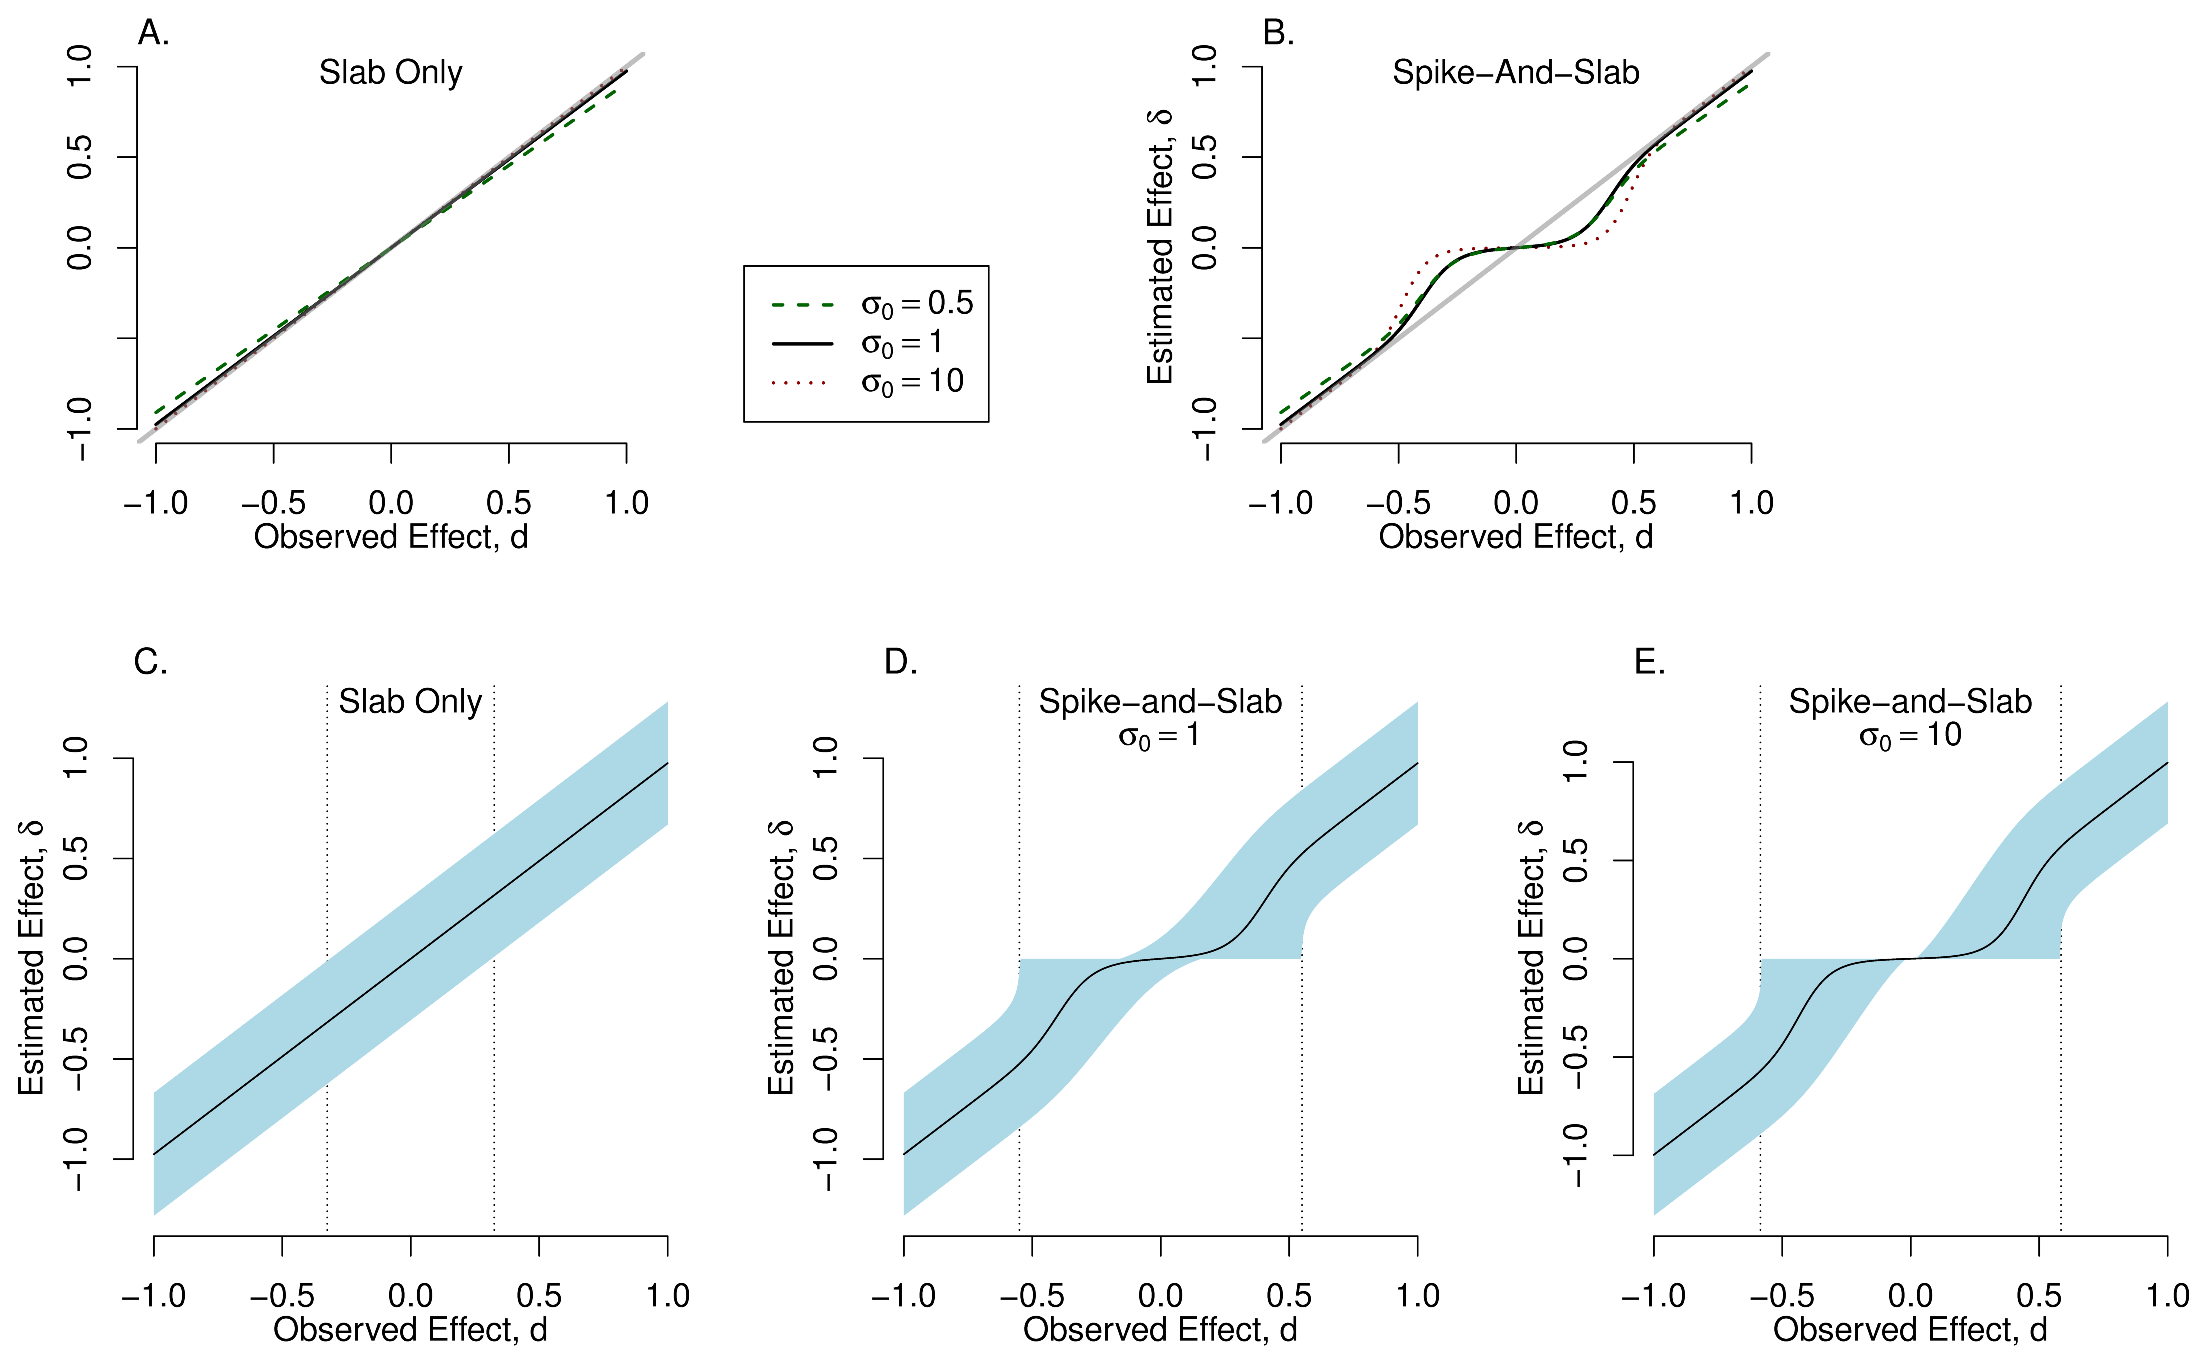
\includegraphics[width=\textwidth]{figs/bi4_fig5}
\caption{A comparison of slab-only ($\calM_1$) and spike-and-slab ($\calM_s$) specifications for a moderate sample size of $N=40$.  \textbf{A-B}: Posterior mean of $\delta$ as a function of $d$ for a few prior settings of $\sigma_0^2$.  The light grey line is the diagonal, and the posterior mean of the slab-only model approaches this diagonal as the prior becomes more diffuse.  The posterior mean in the spike-and-slab model shows {\em adaptive shrinkage} where small values observed values result in greatly attenuated estimates.  \textbf{C-E}: The posterior means with 95\% credible intervals.  The vertical lines denote transition points---the credible interval does not include zero when the observed effect size is more extreme than these points.  The transition points are more extreme for the spike-and-slab specification than the slab-only specification, and this fact is a direct consequence of the point-mass at zero.}
\label{est}
\end{figure}

The unification through spike-and-slab priors highlights similarities and differences between inference from posterior estimation and inference from Bayes factors as they are commonly used in psychology.  The similarities are obvious, both methods are sibling approaches in the Bayes' rule family lineage.  They rely similarly on specification of detailed models including models on parameters (priors), and updating follows naturally through Bayes' rule.  There are differences as well, and the difference we highlight here is that from model specification.  The recommended methods of inference by estimation, say those from Kruschke, rely on priors that preclude spikes at set points such as points of invariance.  The Bayes factor approaches we have developed in \citeA{Guan:Vandekerckhove:2015}, \citeA{Rouder:etal:2009a}, \citeA{Rouder:Morey:2012} and \citeA{Rouder:etal:2012}, place point-mass on prespecified, theoretically important values.  It is this difference in model specification---rather than the difference in inferential statistic---that leads to some of the most salient differences in practice.

\section{Which Model Specification To Use?}
A critical question for researchers is then which model specification to use.  The answer is that the choice depends on the context of the analysis and the goals of the researcher. As a rule of thumb, if zero is a theoretically meaningful or important quantity of interest it makes sense to consider a point mass on zero .  This specification allows one to compute a posterior probability of the theoretically meaningful value.  For instance, in the usual testing scenarios, researchers consider the ``no-effect'' baseline to be qualitatively different than effects.  The spike-and-slab model instantiates this qualitative difference, and in the process license the theoretically useful abstractions of ``effect'' and ``no effect.''  In the context of this goal, of stating evidence for or against effects, it is reasonable and judicious to use a spike-and-slab estimation approach or, equivalently, a Bayes-factor summary of the change in the spike probability.  In some cases, perhaps ones where measurement is a main goal and where the zero value has no special meaning, a slab-only approach may be best.  Researchers in these measurement contexts, however, should avoid drawing inferences about whether or not there are effects in the data as the model specification does not capture such abstractions.  There will be some differences among researchers as to which specification is best in any given context.  These differences should be welcomed as they are part of the richness of adding value in psychological science \cite{Rouder:etal:2016b}.  In all cases, however, researchers should justify their choices in the context of these goals.  

Researchers who consider Bayes factors may worry about their dependence on prior settings especially when compared to estimation with slab-only models.  This worry is assuredly overstated, and a bit of common sense provides for a lot of constraint. It seems to us unreasonable to consider prior settings that are too small or too large as researchers generally know that true effect sizes in psychological experiments are neither arbitrarily small or large.  A lower limit of $\sigma_0$ is perhaps 0.2 as researchers rarely search for effect sizes smaller than this value and the practical value of such small effects will often be low.\footnote{Which is not to say that small effects cannot be \emph{theoretically} meaningful in certain contexts, but we believe interest in very small effects to be generally low.}  Likewise, an upper limit is perhaps 1.0 as the vast majority of effect sizes are certainly smaller than this value and effects much larger than that would often be clear in day-to-day life.     Within these reasonable---if context-dependent---limits, Bayes factors vary but not arbitrarily so.  We have highlighted the Bayes factor values associated with these limits in Figure~\ref{fig:bi4:bf}A as filled circles.  Here the Bayes factors differ from 1.7 to 2.8 or by about 40\%.  This variation is not too substantial, and in both cases the evidence for an effect is marginal.  Such variation strikes us as entirely reasonable and part-and-parcel of the normal variation in research \citeA{Rouder:etal:2016b}.  It is certainly less than other accepted sources such as variation in stimuli, operationalizations, paradigms, subjects, interpretations and the like.

\section{The Potential of Spike-And-Slab Models In Psychology}
We think spike-and-slab priors are going to gain popularity as psychologists develop and adopt new analytic techniques, especially in big-data applications.  Consider applications in imaging where there are a great many voxels or in behavioral genetics where there are a great many nucleotide markers in a SNP array.  It is desirable to consider the activity in any one voxel or the contribution to behavior of any one marker, and the resulting models necessarily have a large numbers of parameters, say with one parameter for each voxel or each marker.  It is in this context, when there are large numbers of parameters especially relative to the sample size, spike-and-slab priors have  become an invaluable computational tool for assessing effects, say which voxels are active or which alleles covary with a behavior.   The seminal article for assessing covariates in this context is \citeA{George:McCulloch:1993}, and recent conceptual and computational advances, say from \citeA{Scott:Berger:2010} and \citeA{Rockova:George:2013}, make the approach feasible in increasing large big-data contexts. 

As an example of big-data applications in psychology, we highlight the recent work of \citeA{Sanyal:Ferreira:2012} who used spike-and-slab priors for fMRI analysis.  These researchers sought to enhance the spatial precision of imaging by improving the spatial smoothing.  Typically, researchers smooth the image by passing a Gaussian filter over it.  Sanyal and Ferreira instead performed a wavelet decomposition where activation is represented as having a location and a resolution.  In this approach there is a separated wavelet coefficient for each resolution and location pairing, and the upshot is a proliferation of coefficients.  Sanyal and Ferreira placed a spike-and-slab prior on these coefficients, and used large values of $\rho_0$, the prior probability that a coefficient is zero.  In analysis, the posterior for many of these coefficients remained dominated by the spike, and could be removed.  When the activation was reconstructed from only the coefficients for which there was substantial mass from the slab, the image had improved quality.  The resulting smoothing was adaptive---it was more smooth where activation was spatially homogenous (say within structures) and less smooth where activation was spatially heterogeneous (say at boundaries).  

\section{Conclusions}
In this paper we provide a unification between two competing Bayesian approaches---that based on the estimation of posterior intervals and that based on Bayes factors.  A salient difference between these two approaches is in model specification.  It is common in estimation approaches to place broad priors over parameters that give no special credence to a zero point.  Common Bayes factor approaches, such as that from Rouder and Morey and colleagues \cite{Rouder:etal:2009a,Rouder:Morey:2012,Rouder:etal:2012,Guan:Vandekerckhove:2015} are closely related to estimation with a prior that has some point mass at zero.  Which model specification a researcher should choose, whether a broad slab or a spike-and-slab, should depend on the context and goals of the analyst. 

\bibliographystyle{apacite}
\bibliography{bi4}


